\documentclass{article}
\usepackage{pdfpages}

\begin{document}

%\title{On the properties of projectile motion and quadratic air resistance}

%\author{Simon Halvdansson}

%\date{\today}

%\maketitle

%\begin{abstract}
%	The functions for projectile motion in a three dimensional space are derived. Some properties of such motion are defined. Numerical approximations and analytical solutions to the effects of one dimensional quadratic air resistance are made and compared to experimental results with small error. Analytical approximations to two dimensional quadratic air resistance are made using a model which separates low, high and split angle trajectories. The equations of motion for these are derived and plotted and compared to numerical integration of the original differential equation.
%\end{abstract}


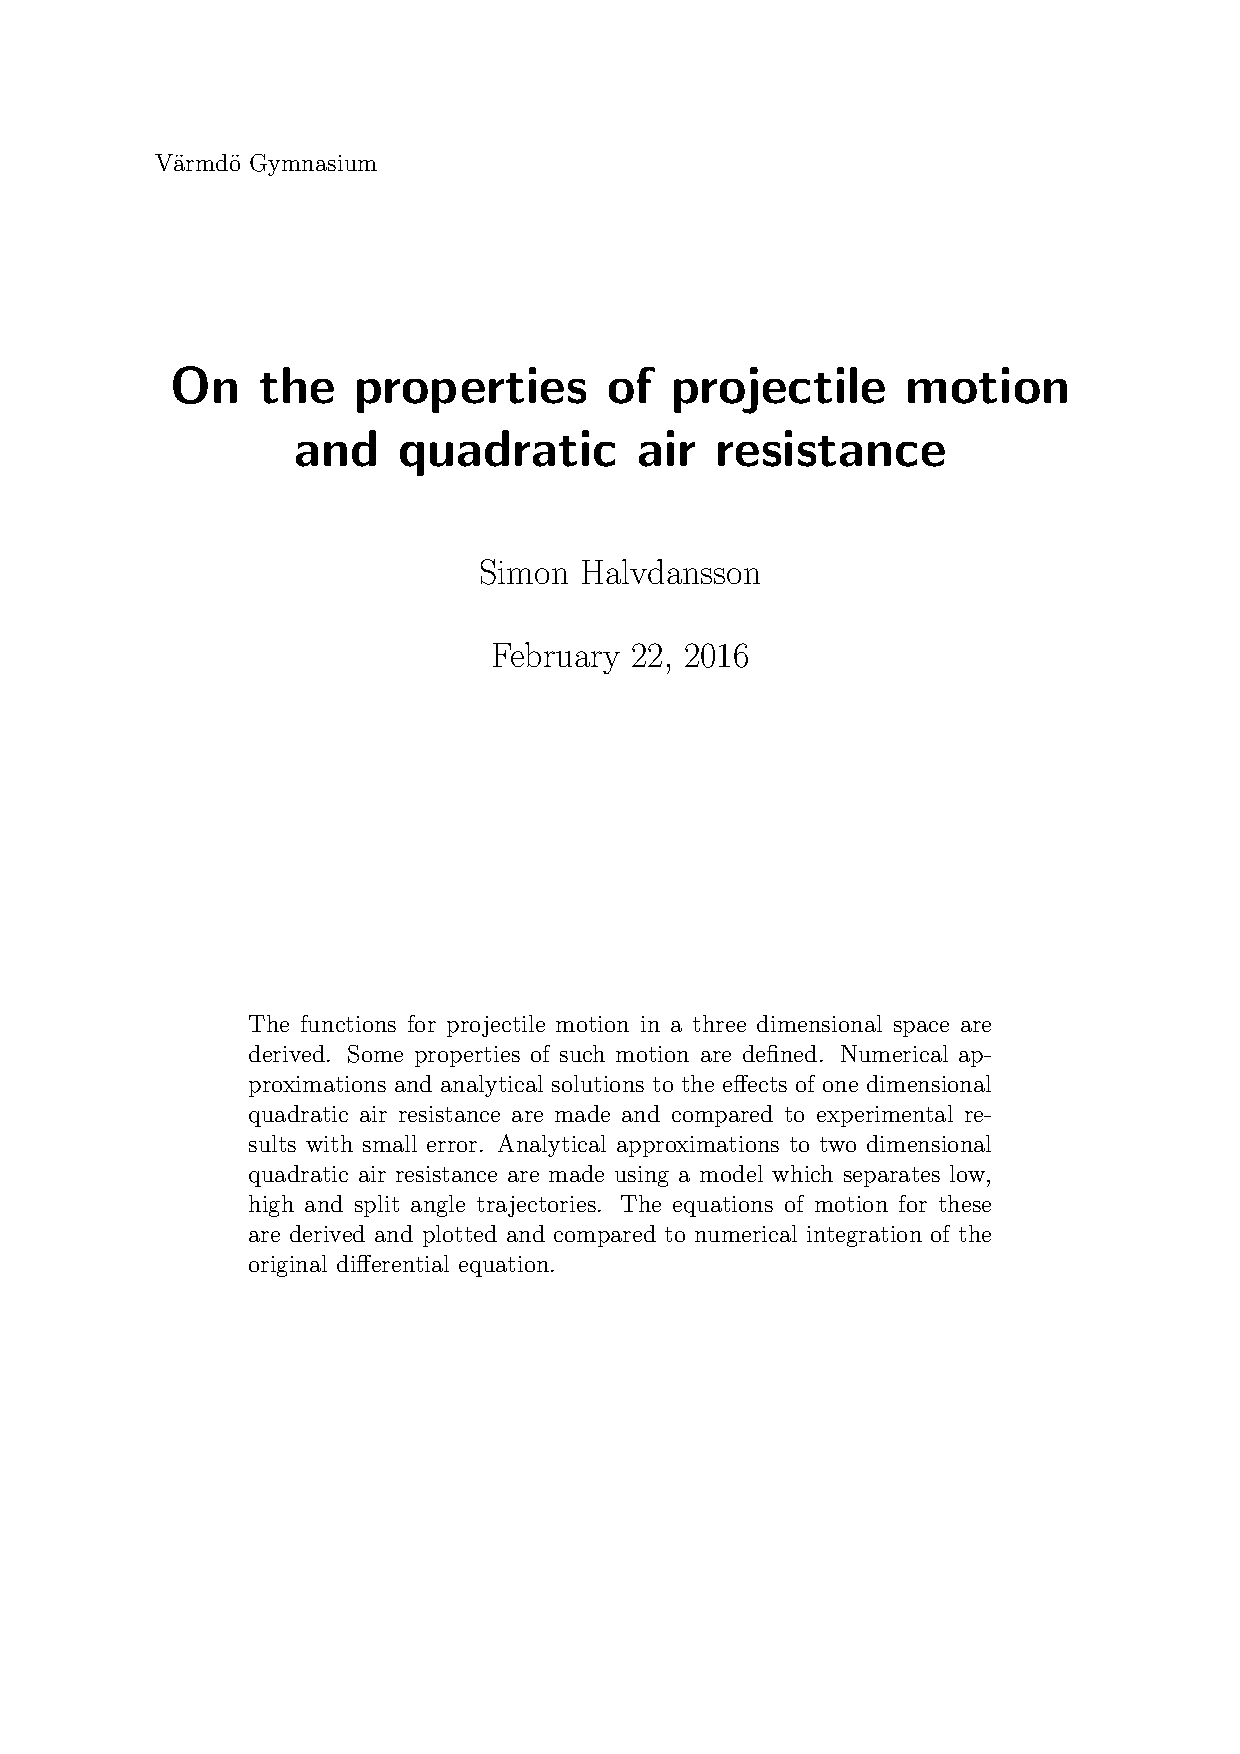
\includepdf[pages=1-]{intro.pdf}
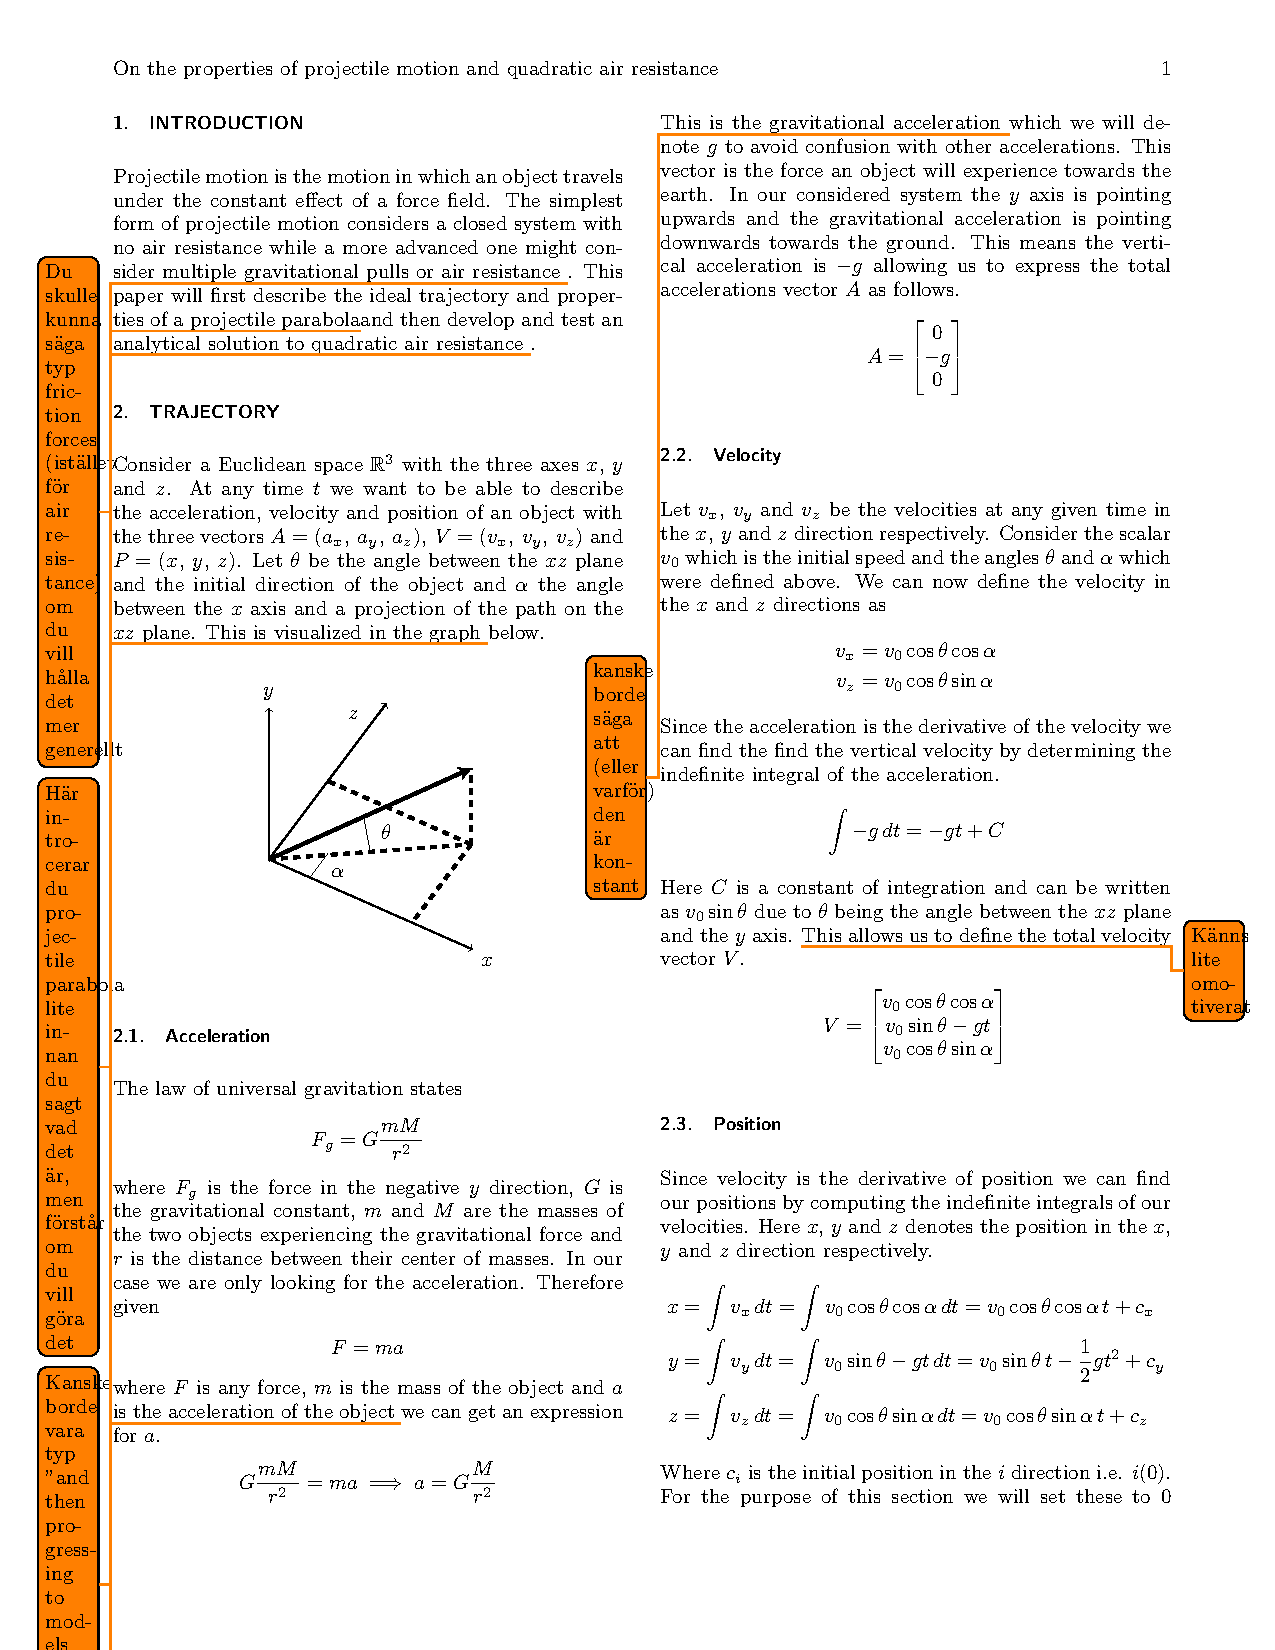
\includepdf[pages=1-]{main.pdf}


\end{document}